\documentclass[conference]{IEEEtran}
\usepackage[utf8]{inputenc}
\usepackage{amsmath,amssymb,graphicx,booktabs}

\usepackage[hidelinks,unicode,pdftitle={Winner's Curse in Validation-Selected Model Merges: A Resampling Study on the Qwen2.5-0.5B Interpolation Grid (ARC, HellaSwag, WinoGrande)},pdfauthor={Dheiver Francisco Santos},pdfkeywords={model merging, winner's curse, validation selection, bootstrap, Qwen2.5},pdfsubject={Preprint, Figshare, doi:10.6084/m9.figshare.35014006}]{hyperref}
\begin{document}

\title{Winner's Curse in Validation-Selected Model Merges: A Resampling Study on the Qwen2.5-0.5B Interpolation Grid (ARC, HellaSwag, WinoGrande)}

\author{\IEEEauthorblockN{Dheiver Francisco Santos, PhD}
\IEEEauthorblockA{Independent Researcher\\
Maceió, Alagoas, Brazil\\
ORCID: https://orcid.org/0000-0002-8599-9436\\
Preprint, Figshare, 2026, \href{https://doi.org/10.6084/m9.figshare.35014006}{doi:10.6084/m9.figshare.35014006}, CC BY 4.0}}

\maketitle

\begin{abstract}
Merge coefficients are usually picked on a small validation set. The maximum over many candidates inflates the winner's validation score (the winner's curse); we did not find a measurement of this inflation for model merging. We measure it on 11 linear interpolations $\theta_t=(1-t)\theta_{\text{base}}+t\,\theta_{\text{inst}}$ between Qwen2.5-0.5B and Qwen2.5-0.5B-Instruct, scored in bfloat16 by the macro average of four benchmarks (ARC-Easy, ARC-Challenge, HellaSwag, WinoGrande; 300 validation and about 1000 test items per task). We select $t$ on 1000 bootstrap resamples of the validation set and compare the validation gain of the selected $t$ over $t=0$ with its test gain. The mean validation gain is $+0.64$~pp and the mean test gain is $+0.17$~pp, a ratio of $3.8$. The mean difference, $+0.48$~pp, comes from simple resampling. The double bootstrap (test items resampled too) gives a 95\% dispersion interval of $[-0.65,+1.77]$~pp, and 67\% of draws are positive. The pure selection bias is $+0.68$~pp. The data are consistent with a winner's curse; its magnitude is unresolved and conditional on bfloat16. One model pair, one grid.
\end{abstract}

\begin{IEEEkeywords}
model merging, winner's curse, validation selection, bootstrap, Qwen2.5
\end{IEEEkeywords}

\section{Introduction}
Weight-space merging is attractive because it needs no training: one picks a few coefficients and keeps the best merged model. In practice the coefficients are chosen by scoring each candidate on a small held-out validation set and reporting the maximum. This is selection from a set of noisy scores, and the maximum of noisy scores is biased upward. In the language of adaptive data analysis, adaptive reuse of a holdout limits how many queries it can answer accurately \cite{dwork2014adaptive}. The question here is quantitative and narrow: \emph{how much of the validation gain of a selected merge coefficient survives on unseen items?}

We study the simplest well-defined case: a one-dimensional grid of 11 coefficients between a base and an instruction-tuned small language model. The validation set is resampled with replacement 1000 times. On each resample the coefficient is selected as a practitioner would, and the validation gain over the unmerged base is compared with the gain of the same coefficient on a fixed test set. Comparing \emph{gains} rather than levels matters: the test split is slightly easier than the validation split, so a level difference mixes selection bias with split difficulty.

\textbf{Contributions.} (i) A resampling estimate of the winner's curse for merge-coefficient selection, with the distribution of selected coefficients. (ii) A gain-based definition that removes the level difference between splits. (iii) A dispersion interval for the optimism that includes the noise of the test set, which shows that the headline ratio is not statistically resolved. (iv) A pure selection-bias estimate in the bootstrap world, which separates selection bias from the validation--test shift.

\section{Related Work}
\textbf{Selection bias and adaptive analysis.} Dwork et al.\ \cite{dwork2014adaptive} study adaptive reuse of a holdout, which limits how many queries it can answer accurately, and give mechanisms (a reusable holdout) that extend that limit. We apply the same concern to a single selection step over a small grid. \textbf{Does selection on a benchmark transfer?} Recht et al.\ \cite{recht2019imagenet} found that accuracies drop on a fresh test set built by the original recipe while the relative order of models is largely preserved, a distribution-shift effect that is related to, but different from, the selection bias studied here. \textbf{Uncertainty in language-model evals.} Miller \cite{miller2024errorbars} recommends reporting standard errors for eval scores; we resample items and use the bootstrap \cite{efron1979bootstrap} for all intervals. Evaluation by log-likelihood of choices follows the common harness convention \cite{gao2021lmeval} on ARC \cite{clark2018arc}, HellaSwag \cite{zellers2019hellaswag} and WinoGrande \cite{sakaguchi2019winogrande}.

\textbf{Merging with validation-selected coefficients.} Model soups pick ingredients and mixing by held-out accuracy \cite{wortsman2022soups}. In task arithmetic and its variants, scaling coefficients are hyperparameters \cite{ilharco2022taskarithmetic,yadav2023ties}. Alternative weightings (Fisher information, prediction-difference minimization) or learned coefficients (AdaMerging) have also been proposed \cite{matena2021fisher,jin2022dataless,yang2023adamerging}. Evolutionary and Bayesian searches optimize merge recipes or checkpoint weights against a development score \cite{akiba2024evolutionary,liu2024checkpointbo}. LoRA composition searches weights with few examples \cite{huang2023lorahub}. Surveys organize methods and applications \cite{yang2024survey}; a large-scale study compares four merging methods across model sizes \cite{yadav2024scale}; toolkits package them \cite{goddard2024mergekit}. In these works the selected score is reported after selection; we did not find a measurement of this inflation for model merging. This paper measures it on one controlled grid. Merged models of the Qwen2.5 family \cite{qwen2024qwen25} are the setting.

\textbf{Author's related work.} The author's technical notes cover neighboring topics in language-model training: model merging for capability composition \cite{santos2026modelmergingfo}, knowledge distillation and self-distillation \cite{santos2026knowledgedisti}, parameter-efficient fine-tuning (LoRA, QLoRA, DoRA) \cite{santos2026parametereffic}, mixture-of-experts training and sparse upcycling \cite{santos2026mixtureofexper}, curriculum learning and data-efficient pretraining \cite{santos2026curriculumlear}, synthetic data generation and self-improvement \cite{santos2026syntheticdatag}, direct preference optimization \cite{santos2026directpreferen}, and RLAIF and Constitutional AI \cite{santos2026rlaifandconsti}. This paper instead reports a controlled held-out measurement. In a different domain, the author's JEPA preprint \cite{santos2026collapseresist} uses a similar controlled-comparison style (identical budgets, several seeds, confidence intervals).

\section{Method}
Let $\theta_0$ and $\theta_1$ be the weights of Qwen2.5-0.5B and its instruct variant, and $\theta_t=(1-t)\theta_0+t\theta_1$ for $t\in\mathcal{T}=\{0,0.1,\dots,1\}$. For a split $D$ and coefficient $t$, let $A_D(t)$ be the macro accuracy over the four tasks. Write $V(t)$ for validation and $A(t)$ for test.

\subsection*{Equations and their meaning}
A bootstrap resample $b$ draws, within each task, $n_k$ validation items with replacement ($n_k$ is that task's validation size), which gives a resampled score $V_b(t)$. The selection rule and the two gains are
\begin{align}
\hat t_b&=\arg\max_{t\in\mathcal{T}} V_b(t),\\
\hat g^{\mathrm{val}}_b&=V_b(\hat t_b)-V_b(0),\qquad
\hat g^{\mathrm{test}}_b=A(\hat t_b)-A(0).
\end{align}
Eq.~(1) is the practitioner's rule (ties go to the smallest $t$). In Eq.~(2) the validation gain is measured on the same resample that picked $\hat t_b$ and the test gain on items that played no role in the choice. Because $t=0$ is in the grid, $\hat g^{\mathrm{val}}_b\ge 0$ always, so its mean is positive even when no coefficient truly helps.

The winner's curse and its summary are
\begin{align}
\hat\Delta_b&=\hat g^{\mathrm{val}}_b-\hat g^{\mathrm{test}}_b,\qquad
\bar\Delta=\tfrac1B\sum_b\hat\Delta_b,\\
\hat R&=\frac{\tfrac1B\sum_b\hat g^{\mathrm{val}}_b}{\tfrac1B\sum_b\hat g^{\mathrm{test}}_b},\quad B=1000.
\end{align}
Eq.~(3) is the optimism of one selection: how much more gain the validation shows than the test confirms. Eq.~(4) restates it as the factor by which the observed validation gain exceeds the realized test gain. Measuring both gains against $t=0$ in their own split removes, to first order, a difficulty offset that is common to all $t$; the level difference $V_b(\hat t_b)-A(\hat t_b)$ does not, and we report it only as a diagnostic.

$\bar\Delta$ mixes two things: the selection bias, and any shift between the validation and test distributions. To isolate the first, let $\bar V(t)$ be the accuracy on the full 300-item validation set (the ``population'' of the bootstrap world) and define the pure selection bias
\begin{equation}
\hat\beta_b=V_b(\hat t_b)-\bar V(\hat t_b).
\end{equation}
It uses no test items. Its mean is the selection bias of the rule in the bootstrap world. The difference $\bar\Delta-\bar\beta$ is minus the validation--test shift of the selected coefficients, $\overline{A(\hat t_b)-A(0)}-\overline{\bar V(\hat t_b)-\bar V(0)}$.

For the uncertainty of $\bar\Delta$ we also run a \emph{double} bootstrap that resamples the test items in the same way (within task, with replacement), so the test gain carries its own sampling noise.

\section{Experimental Protocol}
\textbf{Models.} Qwen2.5-0.5B (base) and Qwen2.5-0.5B-Instruct \cite{qwen2024qwen25}, both Apache-2.0; Hub commits are listed in \texttt{MANIFEST.json} (base \texttt{060db64}, instruct \texttt{7ae5576}). Merging is linear interpolation in fp32 on CPU, then copied to a bf16 model.

\textbf{Data and splits.} ARC-Easy and ARC-Challenge \cite{clark2018arc} (official validation/test splits), HellaSwag \cite{zellers2019hellaswag} and WinoGrande \cite{sakaguchi2019winogrande} (their validation sets partitioned into disjoint validation and test parts with seed 0). Validation has 300 items per task (299 for ARC-Challenge); the test has 1000 per task (967 for WinoGrande), 3967 test items in total. Scoring is multiple-choice log-likelihood in the style of lm-evaluation-harness \cite{gao2021lmeval}: HellaSwag uses length-normalized (per-character) accuracy and WinoGrande partial scoring without normalization. The metric is the unweighted mean of the four task accuracies. Per-item 0/1 outcomes for every configuration are cached, so all resampling reuses a single set of model evaluations.

\textbf{Selection.} The candidate set is the 11-point grid. Selection uses only validation scores; the test set is read once per configuration. This is the same grid and the same split as the LERP experiment of this study; on the full validation set the rule picks $t=0.7$ (macro $0.4961$ versus $0.4953$ at $t=0$).

\textbf{Baselines.} The reference for every gain is $t=0$ (the base model), which is also the better of the two original models on validation. As a no-selection reference we report the mean test gain of a coefficient drawn uniformly from the grid.

\textbf{Statistics.} $B=1000$ bootstrap resamples of the validation set, within task and with replacement, seed 0; the figures in the abstract are means over resamples. Intervals for the optimism are 2.5--97.5 percentiles of the bootstrap distribution. The percentile range of a per-resample quantity is a spread, not a confidence interval of its mean; we call the percentile range of $\hat\Delta_b$ over the double bootstrap (1000 draws, seed 2) a \emph{95\% dispersion interval across resamples}. It describes the spread of one selection, not the uncertainty of $\bar\Delta$; for the mean we report the Monte Carlo standard error. The pure selection bias (Eq.~5) uses the same seed and draw order as \texttt{analyze.py} (seed 0). The hypothesis, fixed in \texttt{experiments/PREREG.md} before any merge was run, is that the validation gain of the selected $t$ exceeds its test gain on this grid; no success threshold beyond that direction was pre-registered. This is a secondary study. Apart from one paired comparison ($t=0.7$ versus $t=0$), we report no p-values. The pre-registration (\texttt{experiments/PREREG.md}) fixed 5,000 bootstrap resamples; the analysis used 2,000 for a single accuracy and 3,000 for paired accuracy differences in \texttt{analyze.py} (5,000 for per-block NLL differences, Articles~7 and 10). The accuracy comparison of Article~10 used $B=5{,}000$; the extra script reproduces the $t=0.7$ versus $t=0$ comparison with that value. The comparison of selected and random coefficients (below) resamples the test items 2,000 times with seed 4 (\texttt{experiments/an\_art08\_selection\_vs\_random.py}). The resampling experiments of this article use $B=1000$ validation resamples, as declared above.

\section{Results}
\textbf{Gains.} Table~\ref{tab:gains} gives the main quantities. The mean validation gain of the selected coefficient is $+0.64$~pp and the mean test gain is $+0.17$~pp, so $\hat R\approx 3.8$. Monte Carlo standard errors of the two means are $0.02$ and $0.01$~pp, so the means are stable across the 1000 resamples; this is not the uncertainty of the underlying population gain. The mean optimism is $+0.48$~pp (means of unrounded values; $0.64-0.17$ rounds to $0.47$). All magnitudes in this section are conditional on bfloat16 evaluation: in fp32 the validation gain of $t=0.7$ over $t=0$ is $+0.34$~pp instead of $+0.08$~pp, measured at three coefficients only, and the grid was not re-evaluated (Sec.~VI). The test gain of the selected coefficient is positive in 53\% of resamples, zero in 18\% (when $t=0$ is selected) and negative in 29\%. A coefficient drawn uniformly from the grid has a mean test gain of $+0.19$~pp, so the two are close ($0.17$ and $0.19$~pp). Holding the 1000 selected coefficients fixed and resampling only the test items (2,000 times, seed 4), the difference between the test gain of the selected coefficient and that of a uniform draw has mean $-0.02$~pp and 95\% percentile interval $[-0.10,+0.07]$~pp (\texttt{results/summary\_art08\_selection\_vs\_random.txt}). We detect no difference larger than about $0.1$~pp from test noise alone; this is not an equivalence test, and it ignores validation-set noise.

\begin{table}[!t]
\caption{Winner's curse on the 11-point LERP grid (1000 validation resamples; gains over $t=0$, in percentage points). Brackets: 95\% dispersion interval (2.5--97.5 percentiles) across resamples of the stated quantity; they are not confidence intervals of the means. The pure selection bias is given for the level version, $V_b(\hat t_b)-\bar V(\hat t_b)$; the gain version, $(V_b(\hat t_b)-V_b(0))-(\bar V(\hat t_b)-\bar V(0))$, has the same mean ($+0.68$), interval $[0.00,+2.09]$ and $\Pr(>0)=0.82$.}
\label{tab:gains}
\centering\small
\begin{tabular}{lc}
\toprule
Quantity & Value \\
\midrule
Mean validation gain $\hat g^{\mathrm{val}}$ & $+0.64$ \\
Mean test gain $\hat g^{\mathrm{test}}$ & $+0.17$ \\
Ratio $\hat R$ & $3.8$ \\
Mean optimism $\bar\Delta$ & $+0.48$ \\
\quad dispersion, validation resamples & $[-0.33,\,+1.68]$ \\
\quad dispersion, double bootstrap & $[-0.65,\,+1.77]$ \\
$\Pr(\hat\Delta_b>0)$, $\Pr(<0)$ & $0.72$, $0.10$ \\
$\Pr(\hat\Delta_b>0)$, double bootstrap & $0.67$ \\
Pure selection bias $\bar\beta$ (Eq.~5, level) & $+0.68$ $[-2.09,\,+3.59]$ \\
Full-validation gain of selected $t$ & $-0.03$ \\
Test gain, double bootstrap & $[-0.72,\,+1.23]$ \\
Level difference (diagnostic) & $-0.23$ $[-2.97,\,+2.75]$ \\
\bottomrule
\end{tabular}
\end{table}

\textbf{Optimism.} The mean optimism is $+0.48$~pp. Its dispersion over validation resamples is $[-0.33,+1.68]$~pp and $\hat\Delta_b>0$ in 72\% of resamples. When the test items are also resampled, the 95\% dispersion interval across resamples is $[-0.65,+1.77]$~pp, which contains zero, and $\Pr(\hat\Delta_b>0)$ over those draws is $0.67$. This interval is the spread of the difference for a single selection, not a confidence interval for $\bar\Delta$; the Monte Carlo standard error of the mean is $0.02$ and $0.01$~pp for the two gains, and the population-level uncertainty of $\bar\Delta$ is not estimated here. The ratio $3.8$ is a ratio of two small means. Its denominator ($+0.17$~pp) lies well inside its own dispersion interval $[-0.72,+1.23]$~pp. The predicted sign holds on average and is consistent with a winner's curse, but we do not establish that the size differs from zero.

\textbf{Pure selection bias.} $\bar\Delta$ compares the resample gain with the gain on a fixed test set, so it also contains the validation--test shift. At $t=0.7$ the full-validation gain over $t=0$ is $+0.08$~pp, while the test gain is $+0.65$~pp. To remove the shift we compute $\hat\beta_b=V_b(\hat t_b)-\bar V(\hat t_b)$ (Eq.~5; \texttt{results/summary\_art08\_pure\_bias.txt}). Its mean is $+0.68$~pp (Monte Carlo SE $0.05$; level version: dispersion interval across resamples $[-2.09,+3.59]$, positive in 67\% of resamples; gain version: same mean, interval $[0.00,+2.09]$, positive in 82\%). The true full-validation gain of the selected coefficient averages $-0.03$~pp, against $+0.17$~pp on the test set. The two estimands answer different questions. $\bar\beta$ is the inflation caused by selection alone, in a world where the 300 validation items are the population. $\bar\Delta$ is the inflation relative to a particular test set; it is smaller ($+0.48$ versus $+0.68$~pp) because the test set happens to favor the large-$t$ coefficients by $0.20$~pp more than the validation set does. Both are estimated under the bootstrap approximation of Sec.~VI.

\textbf{What was actually selected.} Fig.~\ref{fig:gap} shows the distributions of both gains. Table~\ref{tab:choice} gives the frequency of selected coefficients: none dominates. The base model $t=0$ is chosen 18\% of the time, $t=0.7$ (the choice on the full validation set) 17\%, $t=0.4$ and $t=0.8$ 14\% each; $t=0.6$ is never chosen and $t=1.0$ once. The full-validation choice $t=0.7$ yields a test gain of $+0.65$~pp (paired bootstrap interval $[-0.23,+1.52]$, $p=0.149$ with $B=3{,}000$ in \texttt{analyze.py}; \texttt{results/extra\_art07\_art10.txt} gives $[-0.22,+1.51]$, $p=0.147$ with $B=5{,}000$). The interval contains zero, so this gain is not distinguishable from zero. Only 17\% of resamples select a coefficient with a test gain at least that large. The single realized selection was thus a favourable draw relative to the average resample.

\begin{table*}[!t]
\caption{Frequency with which each coefficient is selected over 1000 validation resamples (test gain over $t=0$ in the last row, from the single test set).}
\label{tab:choice}
\centering\small
\setlength{\tabcolsep}{4pt}
\begin{tabular}{lccccccccccc}
\toprule
$t$ & 0 & .1 & .2 & .3 & .4 & .5 & .6 & .7 & .8 & .9 & 1 \\
\midrule
chosen (\%) & 17.9 & 4.0 & 8.9 & 10.3 & 14.3 & 5.6 & 0 & 17.2 & 14.3 & 7.4 & 0.1 \\
test gain (pp) & 0 & $-0.05$ & $-0.41$ & $-0.24$ & $+0.04$ & $-0.03$ & $+0.62$ & $+0.65$ & $+0.49$ & $+0.58$ & $+0.40$ \\
\bottomrule
\end{tabular}
\end{table*}

\begin{figure}[!t]
\centering
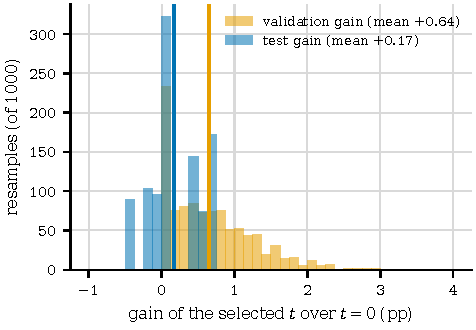
\includegraphics[width=\columnwidth]{figs/fig08b_gain_gap.pdf}
\caption{Histograms, over 1000 validation resamples, of the validation gain (left) and the test gain (right) of the selected $t$ over $t=0$; vertical lines are the means ($+0.64$ and $+0.17$~pp). The mass at zero is the 18\% of resamples that select $t=0$.}
\label{fig:gap}
\end{figure}

\begin{figure}[!t]
\centering
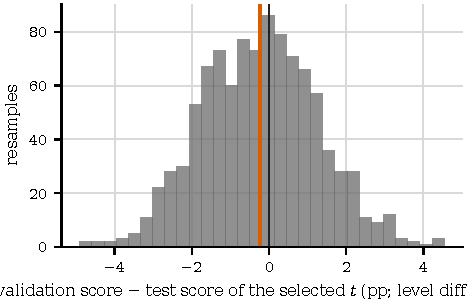
\includegraphics[width=\columnwidth]{figs/fig08_winners_curse.pdf}
\caption{Histogram of the level difference (validation minus test score of the selected $t$; mean $-0.23$~pp), a diagnostic only. It mixes selection optimism with the easier test split, so the negative mean is not evidence against a winner's curse. Fig.~\ref{fig:gap} compares gains instead.}
\label{fig:level}
\end{figure}

\section{Discussion and Limitations}
The measured pattern is consistent with what the winner's curse predicts: the maximum of 11 noisy validation scores sits above the test gain of the same coefficient. A positive optimism whose dispersion interval contains zero means the sample is too small to pin down the factor. With 300 validation items and about 1000 test items per task, the standard error of the test gain is of the same order as the gain. We do not know how the ratio would change with larger sets. We conjecture that the flatness of the response curve over $t$ (all test accuracies lie within $1.06$~pp, all validation accuracies within $1.09$~pp) is why many different coefficients win. We did not test this mechanism. The mean test gain of selection ($+0.17$~pp) is close to that of a random coefficient ($+0.19$~pp; difference $-0.02$~pp, interval $[-0.10,+0.07]$ from test noise alone), so we detect no advantage of validation selection over random choice on this grid. It does not follow that selection is useless on other grids. All evaluations used bfloat16. Re-evaluating validation accuracy in fp32 at $t=0$, $0.7$ and $1$ lowered the macro accuracy by $0.67$, $0.41$ and $0.08$~pp (fp32: $0.4886$, $0.4920$, $0.4845$), a shift of the same size as the differences between coefficients, while the order of the three points did not change and WikiText-2 NLL moved by at most $0.0026$ nats at any $t$ (\texttt{results/fp32\_check\_qwen.txt}). The validation gain of $t=0.7$ over $t=0$ is $+0.08$~pp in bfloat16 and $+0.34$~pp in fp32. The magnitude of the optimism is therefore conditional on bfloat16, and exact accuracy levels are specific to it. Only three points were measured in fp32, the grid was not re-evaluated, and the test items were not re-evaluated either.

\textbf{Threats to validity.} (i) One model pair, one interpolation family, one hardware, four multiple-choice benchmarks, models of $\le0.5$B parameters. (ii) The bootstrap treats the 300 validation items as the population. Each resampled set contains about two thirds of the distinct items of the real one, so the optimism estimated in this empirical world is not an exact estimate for an independent validation set. (iii) The test set is the only out-of-sample reference; its own noise is included only in the double bootstrap. (iv) Gains are compared at the macro level, tasks equally weighted. (v) Benchmark contamination in the pretraining data of the models is possible and was not examined. (vi) The test split is easier than the validation split; the gain-based comparison removes a common offset only approximately, and the shift that remains is the reason we also report the pure selection bias $\bar\beta$.

\section{Conclusion}
On an 11-point base-to-instruct interpolation grid of Qwen2.5-0.5B, the validation gain of the selected coefficient averages $+0.64$~pp against $+0.17$~pp on the test set (about $3.8\times$), and no coefficient dominates the selection. The sign of the winner's curse is consistent with the hypothesis. The pure selection bias is $+0.68$~pp; it is positive by construction in the bootstrap world (a maximum of noisy scores), so it is a property of the procedure, not an independent empirical finding. All magnitudes are conditional on bfloat16. The dispersion interval of the optimism contains zero once test noise is included, so the factor is an estimate, not a settled number. On this grid the post-selection validation score of a merge coefficient is consistent with an overstated gain; a paired test-set gain with an interval is the figure to report.

\section*{Data and Code Availability}
Repository \texttt{artigos-pesos-modelos-pequenos}, git tag \texttt{preprints-v1} (the commit that contains this manuscript and all scripts and caches); the per-item cache is in \texttt{cache/}. Original analysis: \texttt{experiments/analyze.py} (output \texttt{results/summary\_art08.txt}, Fig.~\ref{fig:level}); added computations (double bootstrap, selection counts, random baseline, Fig.~\ref{fig:gap}): \texttt{experiments/an\_art0809\_extra.py} (output \texttt{results/summary\_art0809\_extra.txt}); pure selection bias: \texttt{experiments/an\_art08\_pure\_selection\_bias.py} (seed 0; output \texttt{results/summary\_art08\_pure\_bias.txt}). Single command: \texttt{./run\_everything.sh}. Software: Python 3.9.6, PyTorch 2.8.0, transformers 4.57.6, numpy 1.26.4, datasets 4.5.0; model revisions as in \texttt{MANIFEST.json}. Merging and evaluation ran on Apple Silicon (MPS, bf16); no training is involved, so the only seeds are the data split (0) and the resampling seeds.

\section*{Acknowledgments}
No external funding.

\begin{thebibliography}{99}
\bibitem{dwork2014adaptive} C.~Dwork, V.~Feldman, M.~Hardt \emph{et al.}, ``Preserving statistical validity in adaptive data analysis,'' arXiv:1411.2664, 2014.
\bibitem{recht2019imagenet} B.~Recht, R.~Roelofs, L.~Schmidt, and V.~Shankar, ``Do ImageNet classifiers generalize to ImageNet?'' arXiv:1902.10811, 2019.
\bibitem{miller2024errorbars} E.~Miller, ``Adding error bars to evals: A statistical approach to language model evaluations,'' arXiv:2411.00640, 2024.
\bibitem{efron1979bootstrap} B.~Efron, ``Bootstrap methods: Another look at the jackknife,'' \emph{Ann.\ Statist.}, vol.~7, no.~1, pp.~1--26, 1979, doi:10.1214/aos/1176344552.
\bibitem{gao2021lmeval} L.~Gao \emph{et al.}, ``EleutherAI/lm-evaluation-harness,'' Zenodo, doi:10.5281/zenodo.10256836.
\bibitem{clark2018arc} P.~Clark, I.~Cowhey, O.~Etzioni \emph{et al.}, ``Think you have solved question answering? Try ARC, the AI2 Reasoning Challenge,'' arXiv:1803.05457, 2018.
\bibitem{zellers2019hellaswag} R.~Zellers, A.~Holtzman, Y.~Bisk, A.~Farhadi, and Y.~Choi, ``HellaSwag: Can a machine really finish your sentence?'' in \emph{Proc.\ ACL}, 2019, arXiv:1905.07830.
\bibitem{sakaguchi2019winogrande} K.~Sakaguchi, R.~Le~Bras, C.~Bhagavatula, and Y.~Choi, ``WinoGrande: An adversarial Winograd schema challenge at scale,'' arXiv:1907.10641, 2019.
\bibitem{qwen2024qwen25} Qwen, A.~Yang \emph{et al.}, ``Qwen2.5 technical report,'' arXiv:2412.15115, 2024.
\bibitem{wortsman2022soups} M.~Wortsman, G.~Ilharco, S.~Y. Gadre \emph{et al.}, ``Model soups: Averaging weights of multiple fine-tuned models improves accuracy without increasing inference time,'' in \emph{Proc.\ ICML}, 2022, arXiv:2203.05482.
\bibitem{ilharco2022taskarithmetic} G.~Ilharco, M.~T. Ribeiro, M.~Wortsman \emph{et al.}, ``Editing models with task arithmetic,'' in \emph{Proc.\ ICLR}, 2023, arXiv:2212.04089.
\bibitem{yadav2023ties} P.~Yadav, D.~Tam, L.~Choshen \emph{et al.}, ``TIES-Merging: Resolving interference when merging models,'' in \emph{Proc.\ NeurIPS}, 2023, arXiv:2306.01708.
\bibitem{matena2021fisher} M.~Matena and C.~Raffel, ``Merging models with Fisher-weighted averaging,'' arXiv:2111.09832, 2021.
\bibitem{jin2022dataless} X.~Jin, X.~Ren, D.~Preotiuc-Pietro, and P.~Cheng, ``Dataless knowledge fusion by merging weights of language models,'' in \emph{Proc.\ ICLR}, 2023, arXiv:2212.09849.
\bibitem{akiba2024evolutionary} T.~Akiba, M.~Shing, Y.~Tang \emph{et al.}, ``Evolutionary optimization of model merging recipes,'' \emph{Nat.\ Mach.\ Intell.}, 2025, arXiv:2403.13187.
\bibitem{liu2024checkpointbo} D.~Liu, Z.~Wang, B.~Wang \emph{et al.}, ``Checkpoint merging via Bayesian optimization in LLM pretraining,'' arXiv:2403.19390, 2024.
\bibitem{yang2023adamerging} E.~Yang, Z.~Wang, L.~Shen \emph{et al.}, ``AdaMerging: Adaptive model merging for multi-task learning,'' in \emph{Proc.\ ICLR}, 2024, arXiv:2310.02575.
\bibitem{huang2023lorahub} C.~Huang, Q.~Liu, B.~Y. Lin \emph{et al.}, ``LoraHub: Efficient cross-task generalization via dynamic LoRA composition,'' in \emph{Proc.\ COLM}, 2024, arXiv:2307.13269.
\bibitem{yang2024survey} E.~Yang, L.~Shen, G.~Guo \emph{et al.}, ``Model merging in LLMs, MLLMs, and beyond: Methods, theories, applications and opportunities,'' arXiv:2408.07666, 2024.
\bibitem{yadav2024scale} P.~Yadav, T.~Vu, J.~Lai \emph{et al.}, ``What matters for model merging at scale?'' arXiv:2410.03617, 2024.
\bibitem{goddard2024mergekit} C.~Goddard, S.~Siriwardhana, M.~Ehghaghi \emph{et al.}, ``Arcee's MergeKit: A toolkit for merging large language models,'' arXiv:2403.13257, 2024.
\bibitem{santos2026modelmergingfo} D. F. Santos, ``Model Merging for Capability Composition: A Technical Note,'' Zenodo, 2026, doi:10.5281/zenodo.21610555.
\bibitem{santos2026collapseresist} D. F. Santos, ``Collapse-Resistant Joint-Embedding Predictive Architectures: A Controlled Comparison of SIGReg, VICReg, and EMA,'' Zenodo, v2, 2026, doi:10.5281/zenodo.24223364.
\bibitem{santos2026knowledgedisti} D. F. Santos, ``Knowledge Distillation and Self-Distillation for Language Models,'' Zenodo, 2026, doi:10.5281/zenodo.21610100.
\bibitem{santos2026parametereffic} D. F. Santos, ``Parameter-Efficient Fine-Tuning: LoRA, QLoRA, and DoRA,'' Zenodo, 2026, doi:10.5281/zenodo.21610033.
\bibitem{santos2026mixtureofexper} D. F. Santos, ``Mixture-of-Experts Training and Sparse Upcycling,'' Zenodo, 2026, doi:10.5281/zenodo.21610062.
\bibitem{santos2026curriculumlear} D. F. Santos, ``Curriculum Learning and Data-Efficient Pretraining: A Technical Note,'' Zenodo, 2026, doi:10.5281/zenodo.21610595.
\bibitem{santos2026syntheticdatag} D. F. Santos, ``Synthetic Data Generation and Self-Improvement: A Technical Note,'' Zenodo, 2026, doi:10.5281/zenodo.21610525.
\bibitem{santos2026directpreferen} D. F. Santos, ``Direct Preference Optimization (DPO): A Technical Note,'' Zenodo, 2026, doi:10.5281/zenodo.21609911.
\bibitem{santos2026rlaifandconsti} D. F. Santos, ``RLAIF and Constitutional AI: A Technical Note,'' Zenodo, 2026, doi:10.5281/zenodo.21610280.
\end{thebibliography}

\end{document}
